\section{Funktionelle krav}\label{sec:funktionelle-krav}

\subsection{Use Case Diagram}
Nedenunder ses der et use case diagram lavet ud fra medarbejder-mål tabellen. Use case diagrammet giver et godt overblik over, hvilke opgaver de forskellige aktører udfører mellem aktør og system \cite{visual-paradigm.com}. 

\begin{figure}[H]
    \centering
    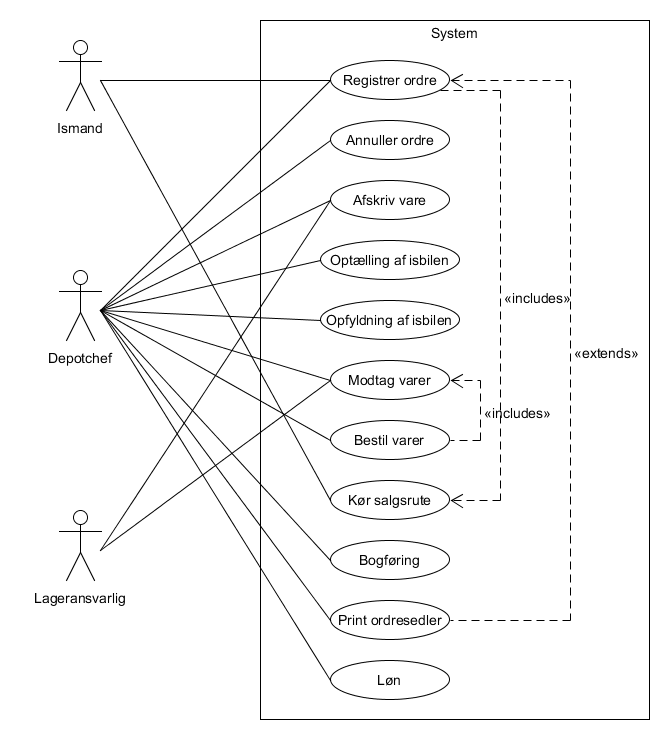
\includegraphics[width=\textwidth]{figures/Forundersøgelse/use_case_diagram.png}
    \caption{Use case diagram}
    \label{fig:use_case_diagram}
\end{figure}

Use Case diagrammet viser at depotchefen står for næsten alle opgaver i virksomheden. Depotchefen udtrykte en interesse for at kunne bruge mindre tid på de mange opgaver han har i løbet af dagen, for så at kunne bruge tid på at køre salgsruter. Da det også primært er depotchefen, der står for de opgaver, som udføres i systemet, er det de Use Cases der vil blive fokuseret på.

\subsection{Fully Dressed} \label{fullydressed}

Herunder ses Fully Dressed Use Casen ‘Automatisk lagerstyring’. Use case 'Automatisk Lagerstyring' er bygget på de tidligere use cases: 'Afskriv vare', fordi den påvirker hvor meget der er på lager. 'Optælling af isbil', som er manuelt arbejde og vil nemt kunne erstattes med automatisk optælling. 'Bestil varer', dette ville gå hånd i hånd med automatisk optælling af bilen. Og til sidst use case 'Modtag varer', fordi systemet skal opdateres med de nye varer der kommer på lager. 

De alternative flows beskrevet i diagrammet er fundet gennem en diskussion, hvor mulige fejl eller forhindringer kan opstå under flowet af handlinger. De alternative flows beskriver, hvordan et system kan fejle undervejs, hvad der er nødvendigt at være forberedt på, og hvordan disse alternative flows kan behandles så systemet ikke stopper, men kan fortsætte Use Casen til ende. Sker det at systemet eller kunden ikke opfører sig som forventet, skal de mulige udfald udtænkes, og sådanne scenarier skal kunne behandles af systemet så vidt muligt.


\begin{longtable}{ |p{120pt}|p{120pt}|p{120pt}| }
    \hline
    \textbf{Use case navn} & Automatisk lagerstyring & \\
    \hline
    \textbf{Aktør} & Depotchefen & \\
    \hline
    \textbf{Præbetingelser} & Et lager med en addresse, penge til at bestille, lager og isbiler er talt op og en smule salgsdata & \\
    \hline
    \textbf{Postbetingelser} & Et lager tilpas fyldt med is & \\
    \hline
    \textbf{Frekvens} & 1 gang om dagen & \\
    \hline
    \textbf{Main Success Scenario} (Flow of events) & \textbf{Aktørhandling} & \textbf{Systemsvar} \\
    \hline
    & 1. Aktøren trykker på "Lager" & 2. Viser lagerbeholdning \\
    \hline
    & 3. Klikker på "Generer lagerplan" & 4. Fil-dialogboks omkring hvor bestillingsplanen skal gemmes. \\
    & & 5. Planen gemmes og sendes automatisk til plan-fanen \\
    \hline
    & 6. Klikker "Åben plan" & 7. Viser bestillingsplanen med mulighed for at kunne rette i den estimerede bestillingsplan. \\
    \hline
    & 8. Klikker "Opret bestilling" & 9. Opretter en bestilling af varer ud fra bestillingsplanen. \\
    \hline
    & 10. Efter nogle dage registreres de ankomne varer i systemet & 11. Lagerstatus opdateret. \\
    \hline
    \textbf{Alternative flows} & 0.1 Udgåede eller ødelagte varer skal afskrives & \\
    \hline
    & 0.2 Afskrevne varer registreres i systemet. & 0.3 Lager status opdateret. \\
    \hline
    & 4.1 Aktøren vil gerne modificere planen, retter det i plan-fanen og gemmer planen & \\
    \hline
    & & 5.1 Der er ikke mere plads på harddisken. \\
    \hline
    & 5.2 Aktøren sletter unødvendige filer for at gøre plads til planen. & 5.3 Gentag trin 5.\\
    \hline
    & & 9.1 Planen er tom. Der kan ikke oprettes en bestilling. Slut på flow. \\
    \hline
\end{longtable}


Understående ses use case 'Automatisk bogføring', som er valgt på baggrund af, at førhen skulle depotchefen sidde og kopiere salgsoplysningerne ned i excel manuelt. Så for at gøre arbejdsgangen nemmere, kan dette gøre automatisk, således at man ikke længere behøver at bruge udnødvendig tid, der kunne have været brugt på andet. 

Nedenfor i fully dressed use casen kan det ses, at selve handlingerne ikke kræver meget tid, hvis det gjort automatisk. Det en relativ hurtig proces, der kun kræver 4-5 nemme steps. 
Hvis tilfædeldet kommer, hvor tallene ikke stemmer overens, med de givende oplysninger, rettes fejlene og trin 1 gentages. 

\begin{longtable}{ |p{120pt}|p{120pt}|p{120pt}| }
    \hline
    \textbf{Use case navn} & Automatisk bogføring & \\
    \hline
    \textbf{Aktør} & Depotchefen & \\
    \hline
    \textbf{Præbetingelser} & ingen & \\
    \hline
    \textbf{Postbetingelser} & bogføring er automatisk færdiggjort i et excel ark & \\
    \hline
    \textbf{Frekvens} & 1 gang om dagen & \\
    \hline
    \textbf{Main Success Scenario} (Flow of events) & \textbf{Aktørhandling} & \textbf{Systemsvar} \\
    \hline
    & 1. Aktøren trykker på "Dashboard" & 2. Viser salgsstatistik \\
    \hline
    & 3. Klikker "Eksporter bogføring" & 4. Systemet exporter en Excel fil med bogføringsdata \\
    \hline
    & 5. Aktøren dobbelttjekker at tallene stemmer overens. & \\
    \hline
    \textbf{Alternative flows} & 5.1 Tallene stemmer ikke overens. & \\
    \hline 
    & 5.2 Ret fejl i registrering og opdater lagerstatus. & \\
    \hline
    & 5.3 Gentag trin 1. & \\
    \hline
\end{longtable}

Efter en vurdering af begge centrale Use Cases, vælges Automatisk Lagerstyring som den endelige use case der fokuseres på. Dette skyldes at det ikke vil være muligt at kunne gennemføre begge use cases på et tilfredsstillende niveau.

\subsection{Kandidattabel}
Nu hvor den centrale Use Cases er valgt, kan der nu laves Kandidatklasser. 
Ved opgaven Automatisk lagerstyring skal \textbf{brugeren} kunne se lagerbeholdningen i \textbf{fryseren}. Ud fra \textbf{salgsstatistik} og tilbud kan den optimale mængde \textbf{varer} bestilles hjem. Det skal være muligt at generere en \textbf{lagerplan}, åbne den, og oprette en \textbf{bestilling} med den. Når de bestilte \textbf{varer} er ankommet skal de registreres i systemet.




\begin{longtable}{ |p{120pt}|p{120pt}|p{120pt}| }\label{fig:Kandidatklasser}
    %\hline %why the fuck doesn't this work?
    \textbf{Kandidat Til Klasse} & \textbf{Vurdering} & \textbf{Konklusion} \\
    \hline
    Køler & Er en fysisk ting der køler is & OUT \\
    \hline
    Sale & Indeholder salgsoplysninger fra et salg ude ved kunden & klasse \\
    \hline
    Product & Indeholder productoplysninger - pris, ID & klasse \\
    \hline
    Customer & Indeholder kundeoplysninger & klasse \\
    \hline
    CustomerOrder & En ordre lavet af en kunde som skal leveres til kunden & klasse \\
    \hline
    DepotOrder & En bestilling af is til depotet & klasse \\
    \hline
    Seller & Indeholder sælgeroplysninger, bliver forbundet med Sale & sale \\
    \hline
    Boss & Indeholder adminstratoroplysninger & klasse \\
    \hline
    DepotPlan & Beskriver hvordan depotet skal ændre sig som sæsonerne gør & klasse \\
    \hline
\end{longtable}
Nu er Kandidatklasserne fundet, og det er nu muligt at opstille en domænemodel af systemet, så basisformen af systemet kan designes, samt forholdene mellem klasserne.


\subsection{Domænemodel}\label{Domainmodel}
Domænemodellen beskriver de relationer klasserne har til hinanden, samt hvilke attributter de indeholder. Her laves domænemodellen ud fra Kandidatklasserne og arkitektur principper.

\begin{figure}[H]
    \centering
    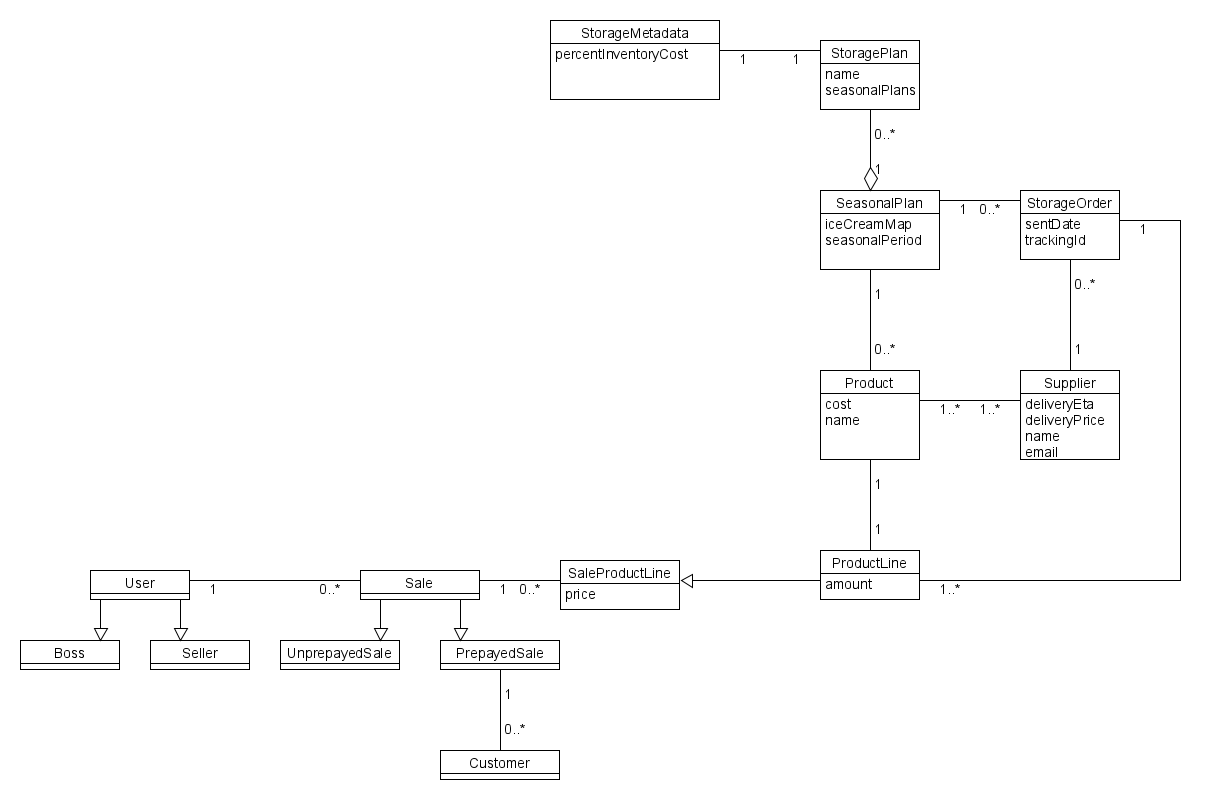
\includegraphics[width=0.9\textwidth]{figures/krav/domain_model.png}
    \caption{Domænemodel}
    \label{fig:domain_model}
\end{figure}

%\section{Ikke-funktionelle krav}